\documentclass{article}

\usepackage{amsmath}
\usepackage{amsthm}
\usepackage[utf8]{inputenc}
\usepackage[portuguese]{babel}
\usepackage{graphicx}

\usepackage{pgffor}

\title{Currículo para Afterschool Online de Análise Real}
\author{}
\date{}

\newtheorem{prop}{Prop}

\addto\captionsportuguese{
	\renewcommand{\proofname}{Dem}
}

\begin{document}
	\maketitle
	
	\section{Metodologia}
	
	Esta iteração de uma Afterschool de Análise Real funcionaria em regime de `clube', adaptado para a internet. Isto é, aos alunos (algures entre 15 e 25, do 9º ao 12º ano) seria providenciado material de estudo (se possível, uma cópia do livro \emph{Introdução à Análise Matemática} do J. C. Ferreira), um local de discussão (um servidor de Discord?), incentivo a discussão (discussões online semanais) e apoio de orientadores. A ideia é que os alunos estudem o material por si mesmos, e o meio servirá para estimular a discussão e entreajuda.
	
	A primeira iteração teria uma duração curta para fazer a experiência, algures entre 6 e 8 semanas. Durante este tempo, seria providenciada uma plataforma de discussão e incentivo regular para participar nela, na forma de problemas dados regularmente, ou em geral, ou em particular. Ver secção \ref{incentivos} para possíveis formas de abordar este tema.
	
	O progresso dos alunos será, em princípio, assíncrono. Isto requer então alguns cuidados. Por exemplo, os exercícios apresentados terão que ser dados em vários `patamares', para qualquer aluno de qualquer nível ter algo em que pensar.
	
	De facto, o currículo será dividido em níveis, cada um destes uma quantidade pequena de matéria, digerível em mais ou menos uma hora de trabalho. Por exemplo, a prova de ingresso (ver abaixo) corresponderá ao nível 1. Cada aluno terá um nível associado. Este nível será maioritariamente usado pelos orientadores para determinar que tipo de exercícios dar no início de uma sessão. Um aluno começará no nível 1 (em princípio, um aluno que entre já `passou' a prova de ingresso, que o qualifica como nível 1).
	
	Numa primeira abordagem, deixaremos os alunos autoavaliar o seu próprio desempenho. A cada nível é fornecida uma quantidade de exercícios -- dependendo do nível e da especificidade do assunto, mas em média seria agradável apontar para pelo menos cinco -- e será sugerido ao aluno que ele `domina um nível' quando consegue resolver confortavelmente todos os exercícios. Para os alunos que estão em dúvida sobre se entendem realmente a matéria, talvez seja boa ideia dar a opção de um monitor os `testar', fazendo uma prova oral.
	
	Idealmente, os exercícios terão diferentes níveis de dificuldade, e possivelmente várias alíneas. Dentro destes, seria boa ideia ter pelo menos um ou dois que são tomados como `protegidos', otimamente os mais difíceis. A estes, não seriam providenciadas dicas, e seria pedido aos alunos que não digam a resposta uns aos outros, apesar de ser encorajada discussão. O objetivo destes é impedir o possível problema de um aluno não se poder testar a si mesmo porque já ouviu a solução a todos os exercícios.
	
	De modo a encorajar o comportamento desejado dos alunos, seria boa ideia criar um `handout' para eles saberem como se comportar. Mantê-lo curto para diminuir o ruído, e indicar as seguintes coisas:
	
	\begin{itemize}
	\item O método de funcionamento do afterschool
	
	\item Encorajar os alunos a conviver no Discord, tanto para falar de matemática como de outros assuntos (há-que encorajar sentido de comunidade!)
	
	\item Indicar onde se pode aceder à lista de exercícios, mencionando que alguns deles são suposto servir como teste e como tal é desejável que eles não contem a solução a outras pessoas (mas é ainda válido tentar resolvê-los em conjunto!).
	
	\item Explicar o funcionamento dos níveis, e indicar o sítio onde eles poderão consultar a que parte do livro corresponde cada nível e reportar o seu progresso. Indicar que, em caso de dúvida, podem fazer perguntas a monitores.
	\end{itemize}

	\section{Servidor}

	Esta secção discute a possível organização do servidor.

	A este servidor, pertenceriam os monitores e os alunos. Opcionalmente, poder-se-ia também deixar o servidor mais ou menos aberto ao público, para que mesmo que aqueles que não terão conseguido entrar possam também usufruir do ambiente. No entanto, especialmente numa primeira abordagem, talvez seja melhor manter o número de alunos mais controlado.

	Usufruir-se-ia do sistema de canais para separar as seguintes funções:

	\begin{itemize}
	\item Discussão geral relacionada com a bibliografia em questão

	\item Discussão geral sobre matemática

	\item Resolução de dúvidas e discussão de exercícios (aviso de spoilers?)

	\item Pelo menos um canal dedicado a ``off-topic'', para não ser só trabalho.
	\end{itemize}

	\section{Incentivos}\label{incentivos}

	De modo a motivar os alunos, faz sentido haver um sistema para manter os alunos interessados e desafiados. A forma natural de o fazer é propor exercícios novos (ou equivalente) regularmente. Situam-se abaixo diversas possibilidades. Não é necessário, e poderá aliás ser excessivo, a implementação de todas.

	\begin{itemize}
	\item Problema da semana. Isto é, cada semana seria proposto um problema (de dificuldade não-trivial) e os alunos seriam encorajados a discuti-lo em grupo. Esta ideia foi inspirada pela forma pelos cursos do AOPS funcionam.

	Este método poderá não ser otimal dada a natureza assíncrona do sistema, que significa que um dado problema poderá ao mesmo tempo ser demasiado à frente para alguns alunos e demasiado atrás para outros. Uma solução a este obstáculo seria dar problemas diferentes a níveis diferentes. Este processo poderia ser mais granularizado, levando a:

	\item Problemas da semana, atribuídos a grupos. Em vez de dar um problema geral para todos, dividir os alunos segundo algum critério (podendo até deixar os alunos agrupar-se naturalmente) e atribuir um problema adequadamente escolhido a cada grupo. Este método é mais trabalho, requerendo atenção mais ou menos individual, mas é mais robusto.

	\item Problemas da semana, autoatribuídos por grupos. Isto é semelhante à ideia anterior, mas em vez de problemas serem atribuídos individualmente, é proposta uma lista de problemas e cada grupo escolhe um problema para resolver.

	\item `Bounties'. Isto é, ocasionalmente sugerir um problema sobre um certo assunto, e dar algum género de recompensa a quem enviar uma solução correta.

	\item Exposições. Isto é, sugerir aos alunos que enviem soluções de exercícios particularmente inspiradas, provas alternativas de teoremas ou formas interessantes de visualizar coisas, e expô-las a todos, dando destaque às melhores. Com alguma sorte, isto incentiva também os alunos a pensar um pouco fora da caixa e ver coisas que não veriam de outra forma. Aliás, com alguma sorte, até nós orientadores poderemos aprender alguma coisa!
	\end{itemize}
	
	\section{Prova de ingresso}
	
	Para a prova de ingresso, é esperado que um aluno leia as seguinte páginas. (As fotos serão substituídas por scans mais legíveis.)
	
	\foreach \n in {1,...,7}{
		\includegraphics[width=\linewidth]{pg\n}
		\newpage
	}
	
	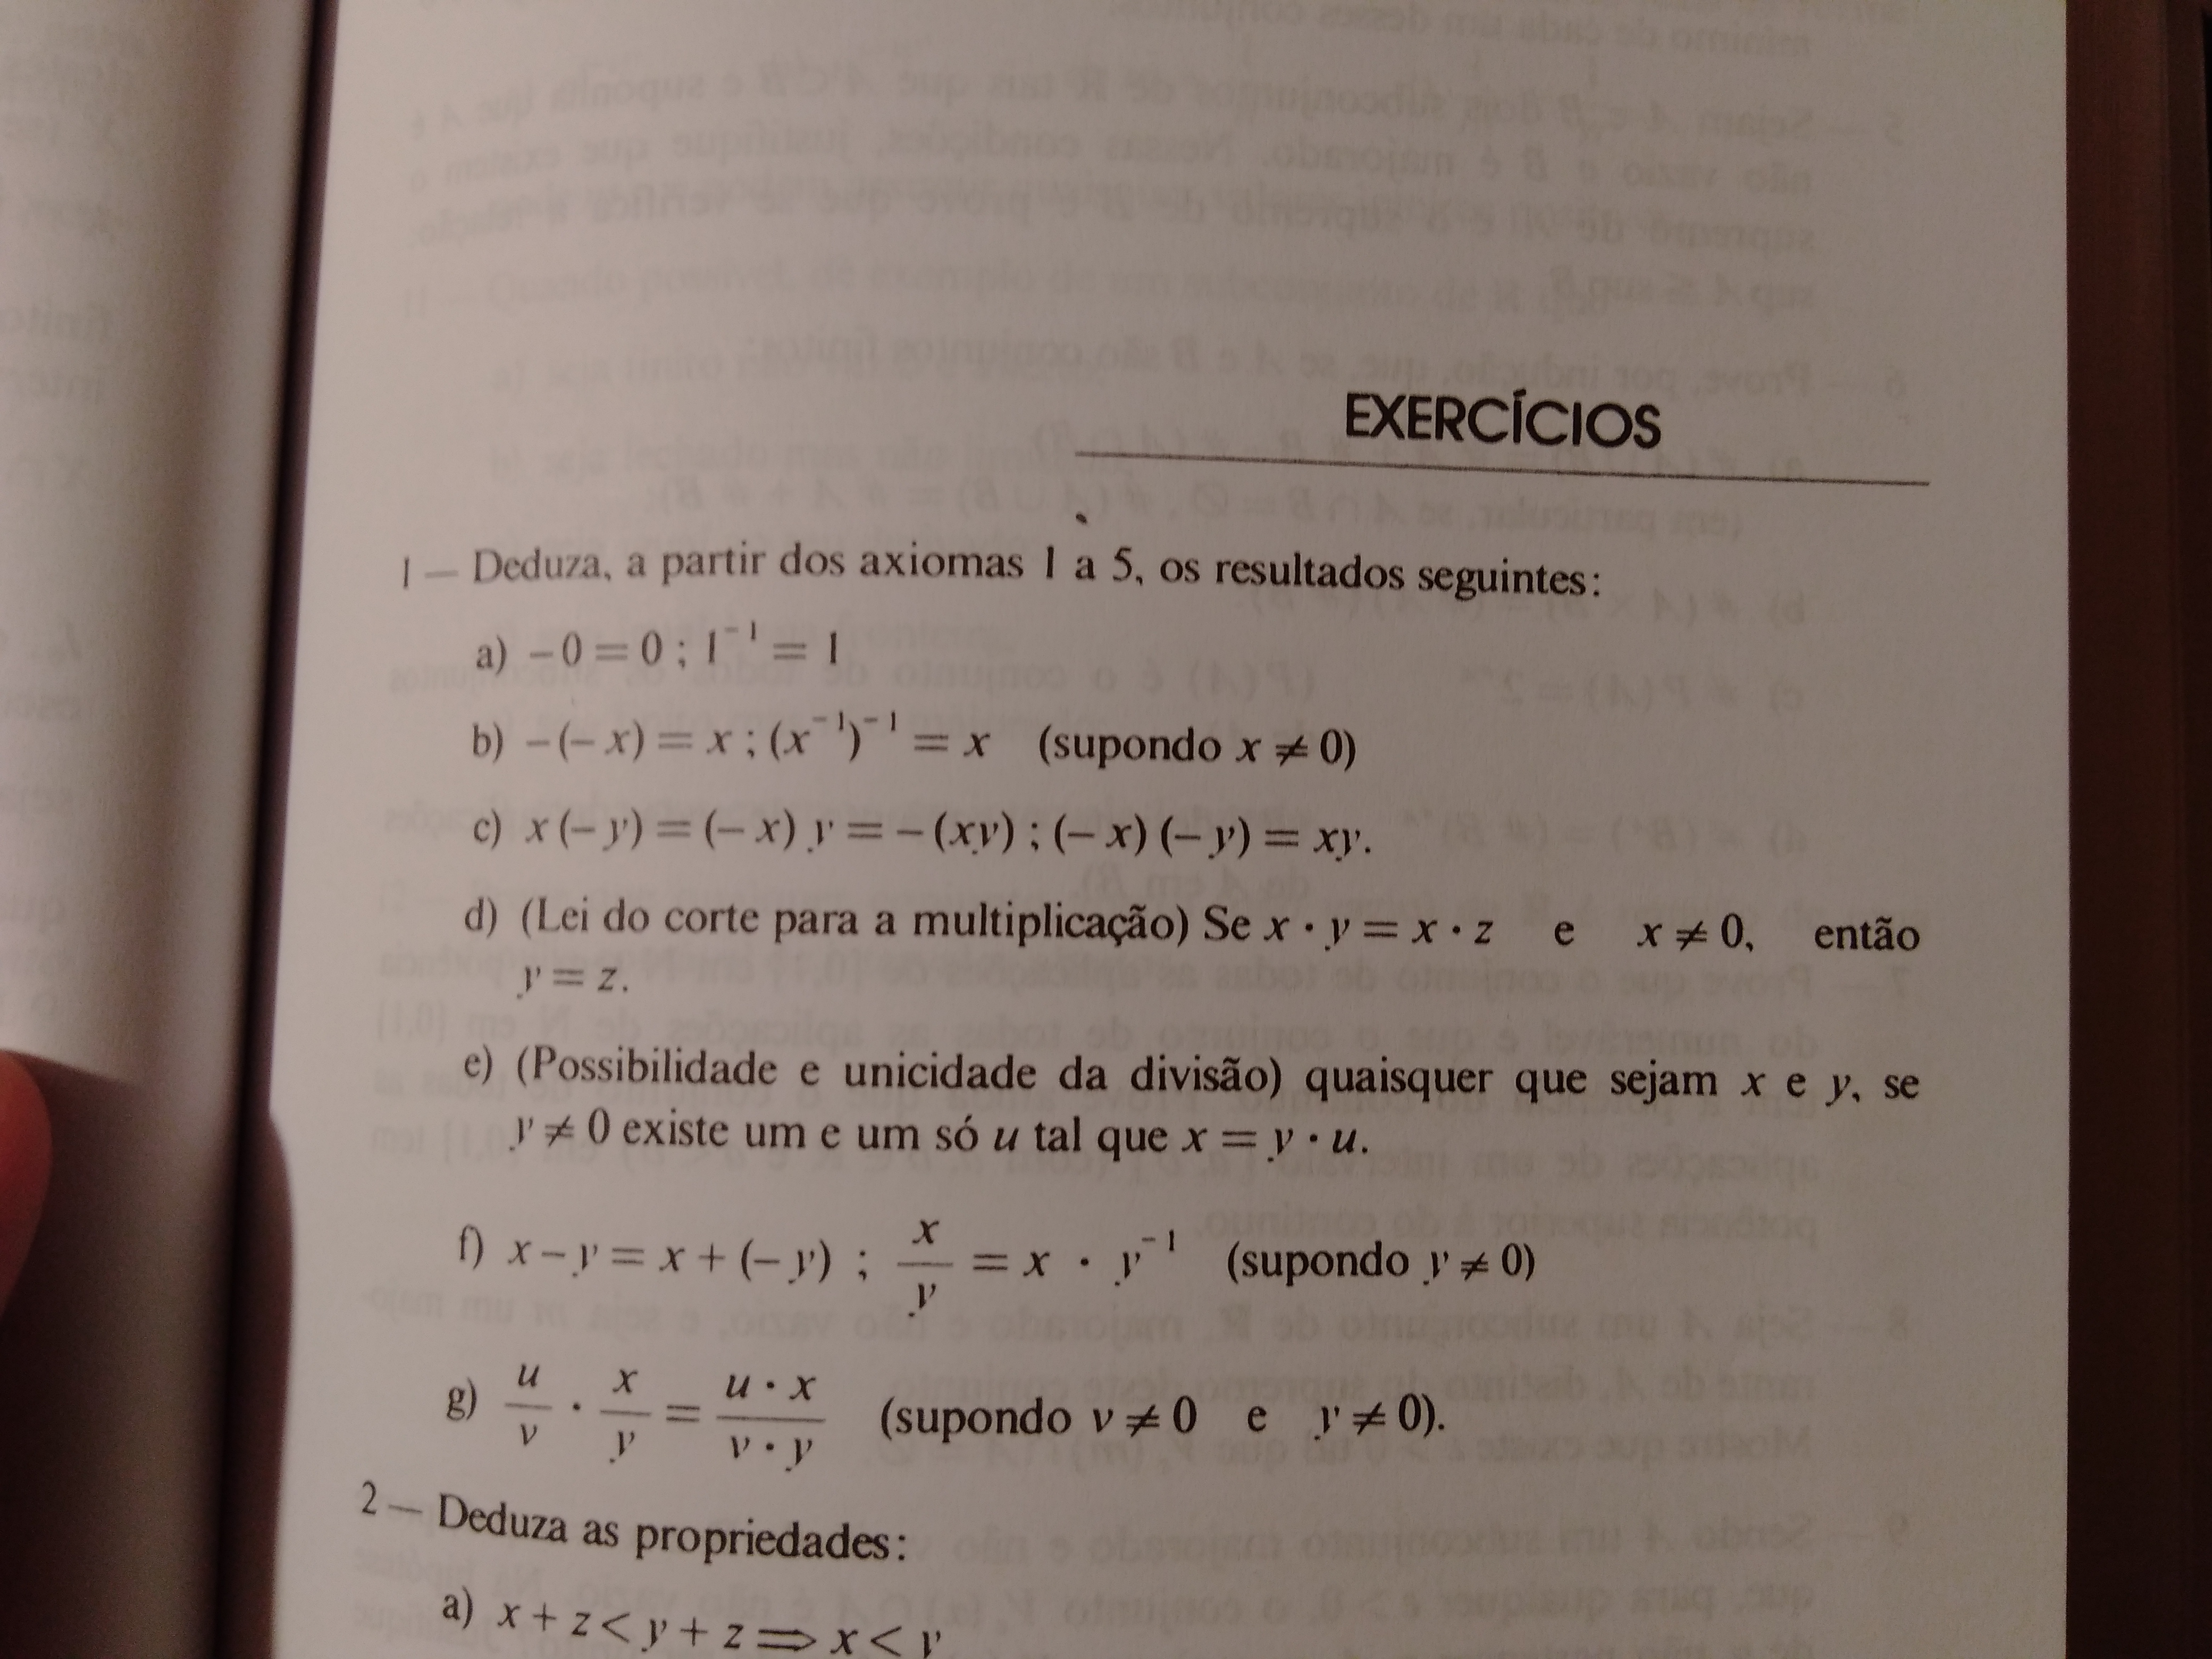
\includegraphics[width=\linewidth]{ex1}
	\newpage
	
	Solicita-se que os alunos submetam um ou mais dos seguintes, como prova de ingresso:
	
	\begin{itemize}
	\item Solução parcial ou total do exercício 1, acima
	
	\item Resumo do capítulo acima, completo com demonstrações. Preferível se as demonstrações forem pelas palavras próprias do aluno. Pontos extra por demonstrações que não são apenas as demonstrações do livro escritas por outras palavras.
	
	\item Qualquer outra coisa que o aluno deseje submeter, desde que mostre uma capacidade de interpretar, pensar e demonstrar coisas.
	\end{itemize}
	
	\section{Níveis}
	
	A seguinte enumeração dos níveis está organizada da forma:\\
	Número. Parágrafo associado; Exercício associado.
	
	Para um aluno completar um nível, é esperado que leia o parágrafo respetivo e saiba resolver o exercício associado.
	
	Estão marcados alguns níveis com asteriscos. Estes são níveis que talvez mereçam alguma revisão, visto que o seu conteúdo poderá ser particularmente difícil e os alunos talvez careçam de contexto para os conceitos introduzidos.
	
	\begin{enumerate}
	\item I.1.1 Axiomas de um corpo; Ex 1
	
	\item I.1.2 Axiomas de ordem; Ex2
	
	\item I.1.3 Números naturais, inteiros e racionais; Ex3 *
	
	\item I.1.4 e I.1.5, Axioma do supremo; Ex4 e Ex5
	
	\item I.1.6 Cardinalidades; Ex6 e Ex7
	
	\item I.2.1, I.2.2, I.2.3 Conceitos topológicos; Ex8 até Ex11
	
	(Exercício bónus: Ex12)
	
	\item II.1.1 Sucessões; Ex1
	
	\item II.1.2 Limite; Ex2 e Ex3
	
	\item II.1.3 Sucessões limitadas e sucessões de Cauchy; Ex4
	
	\item II.1.4 A reta acabada; (Por determinar)
	
	\item II.1.5 (Primeira metade) Algumas operações com limites; Notação `O-grande' e `o-pequeno'; Ex5
	
	\item II.1.6 (Segunda metade) Exponenciais reais; (Por determinar)
	
	(Exercícios bónus: Ex6 até Ex11)
	\end{enumerate}
	
	\section{Problemas em aberto}
	
	Esta secção é dedicada a alguns problemas que poderão surgir, e para os quais vale a pena tentar pensar numa solução.
	
	\begin{enumerate}
	\item Apesar de se ter mandado fora a premissa que o progresso dos alunos está sincronizado, continua subjacente a ideia de que o progresso é linear. No entanto, há a possibilidade de certos temas não dependerem diretamente uns dos outros, formando então um grafo dirigido acíclico de níveis em vez de uma sequência. Por exemplo, um aluno poderá não precisar de saber derivadas antes de aprender o que é o integral, juntando-se os dois ramos quando surge o teorema fundamental do cálculo.
	
	No entanto, seria trabalhoso não só desenhar o grafo (visto que requer um conhecimento profundo do livro que talvez só surja com mais iterações a usar o mesmo) como seria talvez complicado encontrar uma interface para os alunos verem e submeterem os seus níveis. Como tal, talvez esta ideia seja melhor guardada para uma iteração futura.
	
	\item O que fazer quando a auto-reportação do progresso de um aluno falha? Como deve um monitor reagir quando acha que um aluno está a sobre-reportar o seu progresso? Parece injusto mandar o aluno alguns níveis abaixo, não só pelo perigo do que isto possa causar à motivação do aluno em causa, como porque o monitor pode estar simplesmente a avaliar mal. Será talvez a melhor abordagem não fazer nada, sem ser talvez recomendar ao aluno para rever as bases?
	
	Não tenho solução recomendada para isto e agradeço opiniões.
	\end{enumerate}

\end{document}